
\documentclass[12pt, letterpaper]{report}

\title{The Final Report}
\author{Wally Yang, Tina Liang, Wei Zong, Chuwen Sun, Xingyu Yan}
\date{\today}

\usepackage[margin=1in]{geometry}

\usepackage{amsmath}
\setlength{\jot}{12pt} % set the vertical spacing between lines

\usepackage{minted}
\usepackage{xcolor}
\definecolor{monokaibg}{HTML}{272822}

\definecolor{codegreen}{rgb}{0,0.6,0}
\definecolor{codegray}{rgb}{0.5,0.5,0.5}
\definecolor{codepurple}{rgb}{0.58,0,0.82}
\definecolor{backcolour}{rgb}{0.95,0.95,0.92}

\usepackage{amssymb}
\def\ojoin{\setbox0=\hbox{$\bowtie$}%
  \rule[-.02ex]{.25em}{.4pt}\llap{\rule[\ht0]{.25em}{.4pt}}}
\def\leftouterjoin{\mathbin{\ojoin\mkern-5.8mu\bowtie}}
\def\rightouterjoin{\mathbin{\bowtie\mkern-5.8mu\ojoin}}
\def\fullouterjoin{\mathbin{\ojoin\mkern-5.8mu\bowtie\mkern-5.8mu\ojoin}}

\usepackage{graphicx}

\usepackage{multirow}

\begin{document}
\maketitle

\section{Database Description}

\begin{enumerate}
  \item ER-model of the Database Design

    \begin{center}
      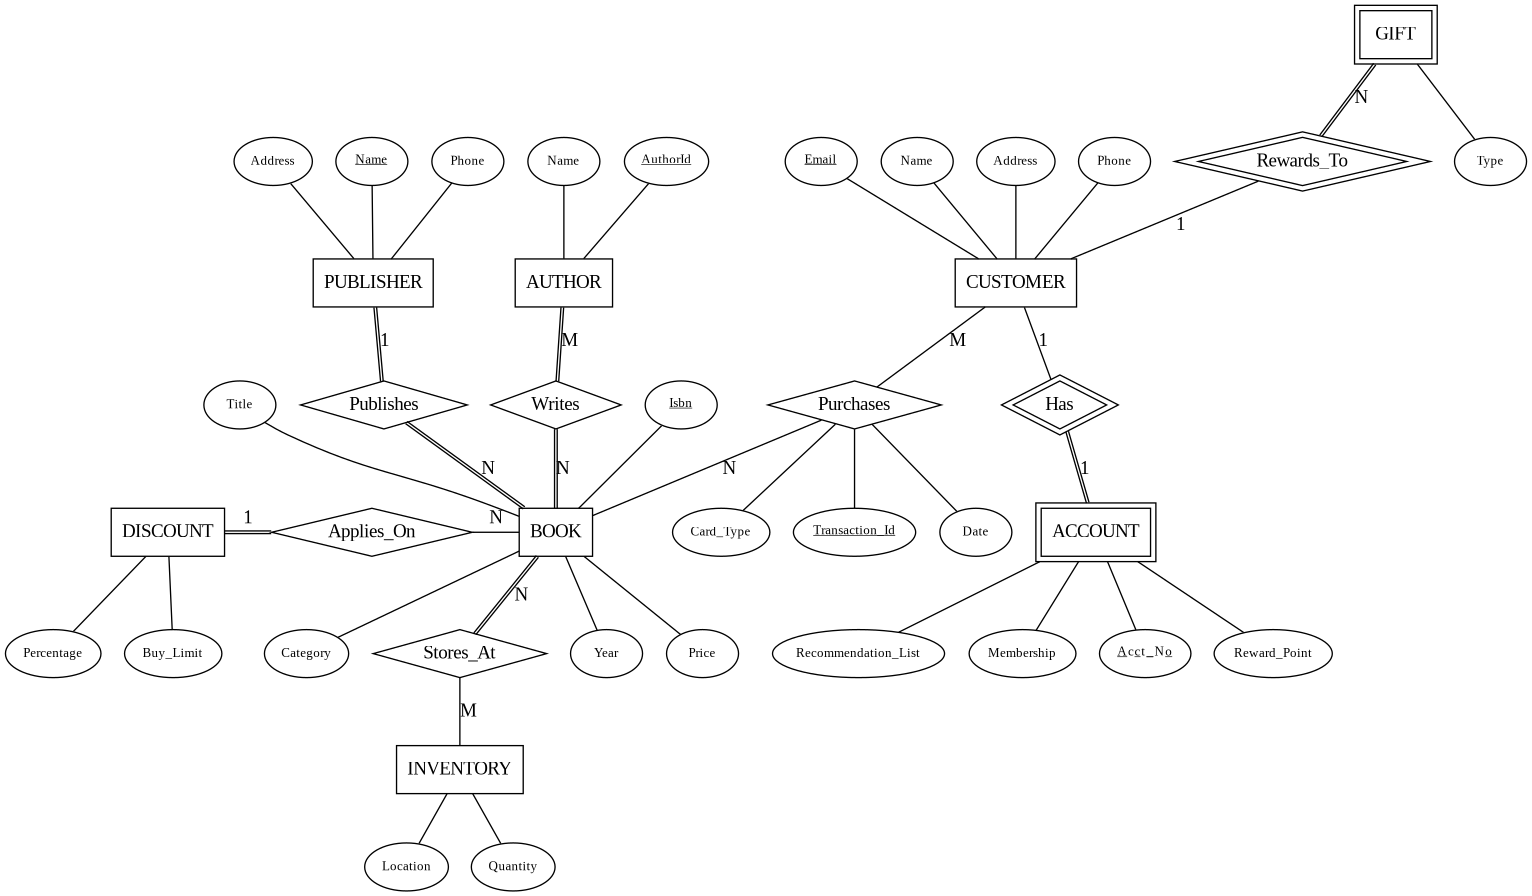
\includegraphics[width=\linewidth]{ER}
    \end{center}

    \pagebreak

  \item Relational Schema for the Database

    \begin{center}
      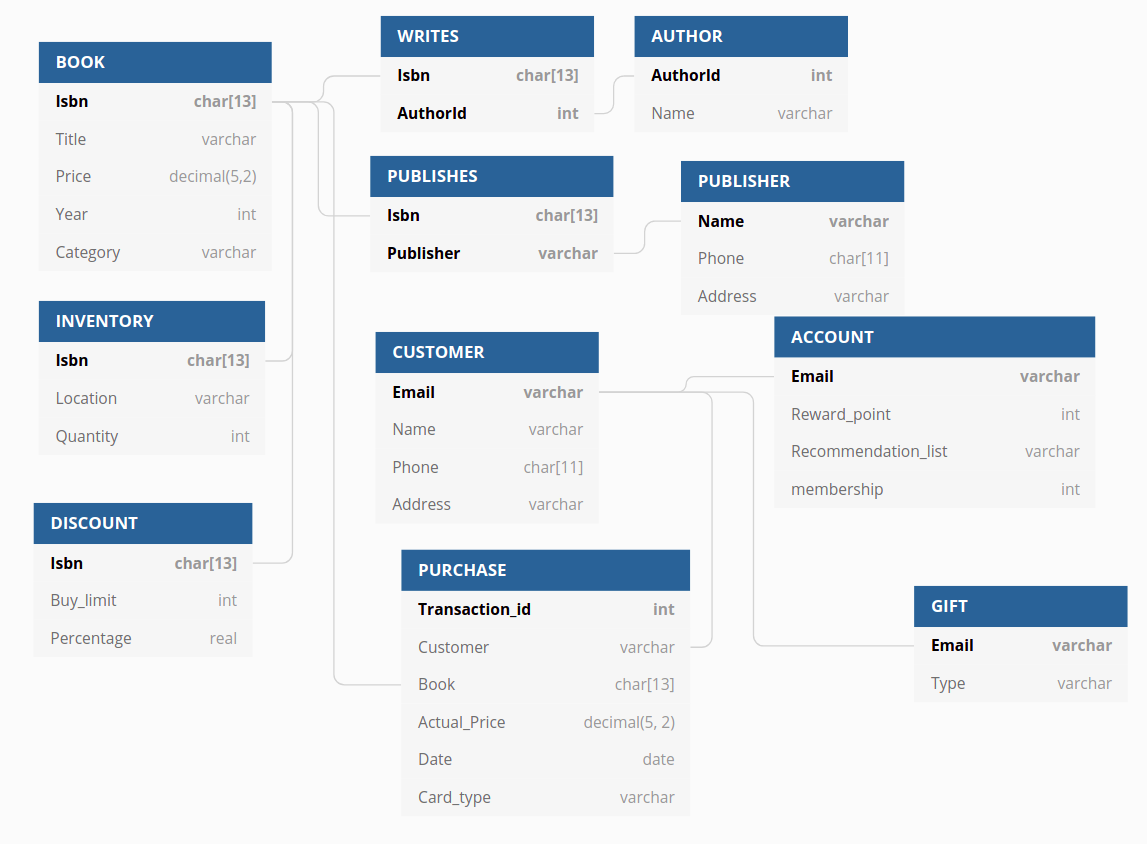
\includegraphics[width=\linewidth]{RelationalSchema}
    \end{center}

    The bold field refers to the primary keys of the relational schema

  \item Levels of normalization for each table:
    All tables achieve BCNF.

  \item Indices for the Database

    We chose the Tree-based index for our BOOK table since the tree-based index is good for looking up values based on range tests. It will speed up our queries when we want to retrieve the book based on the range of the year or the range of the price. Also it is not too bad for looking up values based on equality tests, so it also can slightly speed up our queries when we are trying to look up books based on the titles, categories, authors, and publishers.

  \item Views for the Database

    \begin{itemize}
    \item View A

      Description: This view is able to show all the titles and their dates of purchase made by each customer. And this could be useful to make book recommendations for a customer by looking at his or her purchase history.

      Relational algebra expression:
      \begin{align*}
        &\textit{R1} \leftarrow \textit{PURCHASE} \bowtie_{\textit{Customer} = \textit{Email}} \textit{Customer}\\
        &\textit{R2} \leftarrow \textit{BOOK} \bowtie_{\textit{Isbn} = \textit{Book}} \textit{R1}\\
        &\textit{Result} \leftarrow \pi_{\textit{Name, Title, Date}}\textit{R2}
      \end{align*}

      \inputminted[
      style=monokai,
      bgcolor=monokaibg,
      linenos]
      {sql}{Section1/view_a.sql}

      Sample output:
      \begin{table}[htbp]
        \centering
        \begin{tabular}{| c | c | c |}
          \hline
          Luqman Finnegan	& OCP:	& 07/01/16\\
          & Oracle9i Certification Kit &\\
          \hline
          Phebe Christian	& SQL Server 2000  & 09/16/18\\
          & for Experienced DBA's &\\
          \hline
          Charlie Dolan	& The Data Warehouse Toolkit: & 07/20/18\\
          & The Complete Guide to Dimensional Modeling &\\
          \hline
          Kiya Mcguire & How To Do Everything with Your Tablet PC	& 01/26/19\\
          \hline
          Amal Terrell & Data Mining: & 06/15/17\\
                 & Practical Machine Learning Tools &\\
                 &and Techniques with Java Implementations &\\
          \hline
        \end{tabular}
      \end{table}

    \item View B

      Description: This view is able to show the total number of books purchased by each customer. And this could be useful to see if this customer deserves a gift by making a certain amount of purchases in this store.

      Relational algebra expression:
      \begin{align*}
        &\textit{R1} \leftarrow \textit{PURCHASE} \bowtie_{\textit{Customer} = \textit{Email}} \textit{Customer}\\
        &\textit{Result} \leftarrow _{\textit{Customer}}\mathcal{F}_{\textit{COUNT Book}}(\textit{R1})
      \end{align*}


      \inputminted[
      style=monokai,
      bgcolor=monokaibg,
      linenos]
      {sql}{Section1/view_b.sql}

      Sample output:
      \begin{table}[htbp]
        \centering
        \begin{tabular}{| c | c |}
          \hline
          Ahmed.12@osu.edu & 1\\
          \hline
          Christian.2@osu.edu	& 1\\
          \hline
          Dolan.3@osu.edu	& 1\\
          \hline
          Finnegan.1@osu.edu	& 1\\
          \hline
          Firth.9@osu.edu	& 1\\
          \hline
        \end{tabular}
      \end{table}

    \end{itemize}

  \item Sample Transactions for the Database

    \begin{itemize}
      \item Transaction A

        Description:
        The customer adds a book to a order and update the book quantity in the inventory

        \inputminted[
        style=monokai,
        bgcolor=monokaibg,
        linenos]
        {sql}{Section1/trans_a.sql}

      \item Transction B

        Description:
        A certain amount(10) of books(Isbn: 616601654) transmitted from one inventory(warehouse) to another(in-sotre)

        \inputminted[
        style=monokai,
        bgcolor=monokaibg,
        linenos]
        {sql}{Section1/trans_b.sql}

      \item Transaction C

        Description:
        Customer redeem 100 reward points to a keychain

        \inputminted[
        style=monokai,
        bgcolor=monokaibg,
        linenos]
        {sql}{Section1/trans_c.sql}

    \end{itemize}

\end{enumerate}

\pagebreak

\section{User Manual}
\begin{enumerate}
\item Database Description

  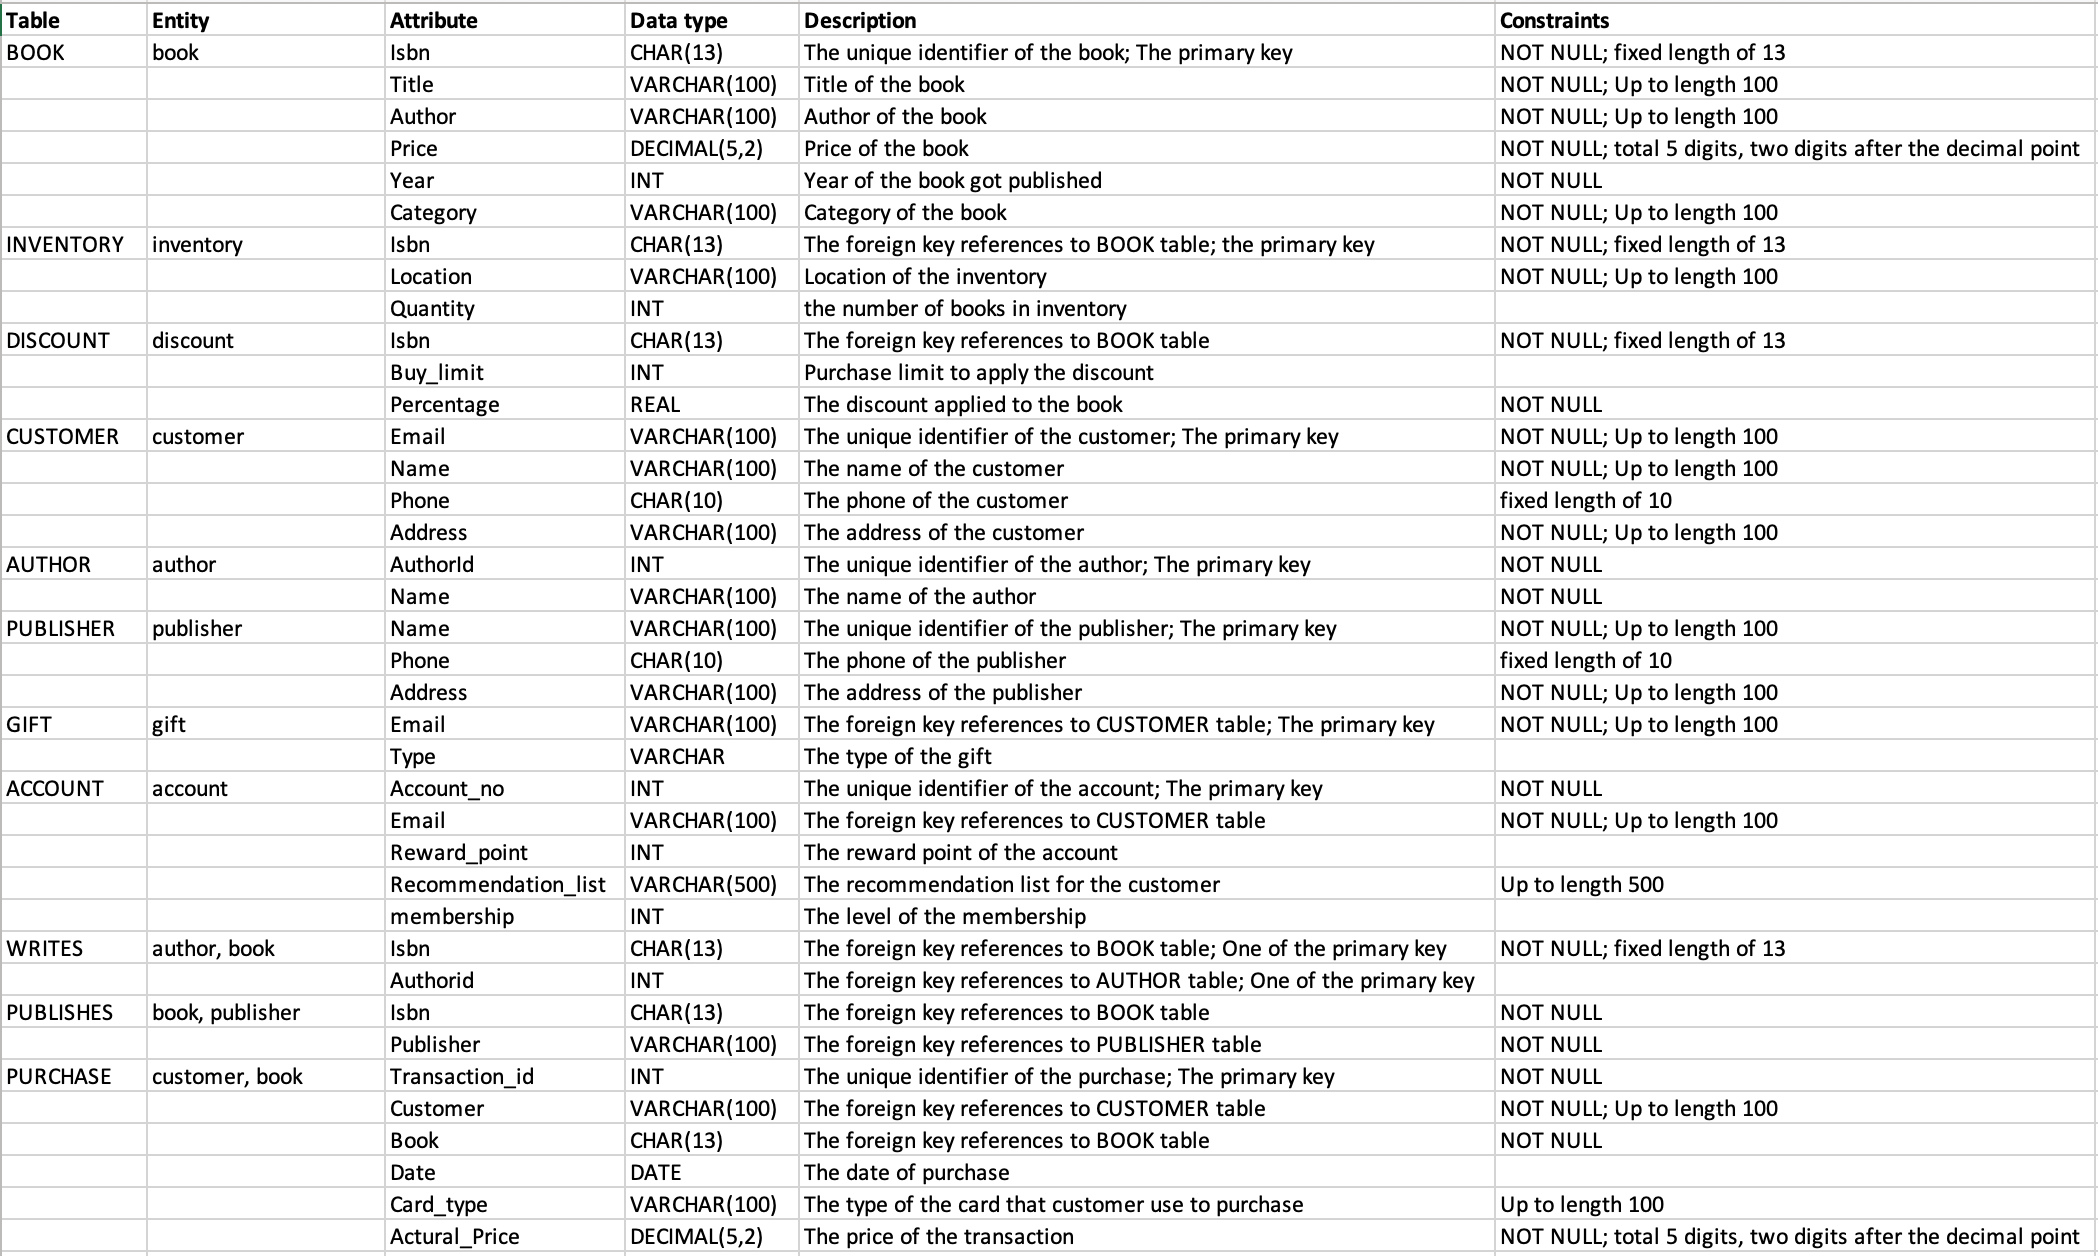
\includegraphics[width=\linewidth]{Section2/description}

\item Sample SQL Queries

  \begin{enumerate}
  \item Find the titles of all books by Pratchett that cost less than \$10

    Return a table that contains the title of that books written by Pratchett and cost less than \$10

    \begin{align*}
      &\mathit{R1} \leftarrow \mathit{BOOK} * \mathit{WRITES} * \mathit{AUTHOR}\\
      &\mathit{R2} \leftarrow \sigma_{\mathit{Name} = \textit{Terry Pratchett}}(R1)\\
      &\mathit{RESULT} \leftarrow \pi_{\mathit{Title}, \mathit{Name}}(\mathit{R1})
    \end{align*}

    \inputminted[
    style=monokai,
    bgcolor=monokaibg,
    linenos]
    {sql}{Section2/query_a.sql}

  \item Give all the titles and their dates of purchase made by a single customer

    Return a table that contains the title and date of the purchases made by a single customer

    \begin{align*}
      &\textit{BOOKS} \leftarrow \textit{BOOK} \bowtie_{\textit{Isbn} = \textit{Book}} (\sigma_{\textit{Customer}=\textit{Email}}(\textit{PURCHASE}))\\
      &\textit{RESULT} \leftarrow \pi_{Title, Date} (\textit{BOOK})
    \end{align*}

    \inputminted[
    style=monokai,
    bgcolor=monokaibg,
    linenos]
    {sql}{Section2/query_b.sql}

  \item Find the titles and ISBNs for all books with less than 5 copies in stock

    Return a table that contains the title and ISBN for all books with less than 5 copies in inventory

    \begin{align*}
      &\textit{STOCK(Isbn, Quantity)} \leftarrow _{\textit{Isbn}}\mathcal{F}_{\textit{SUM Quantity}}(\textit{INVENTORY})\\
      &\textit{RESULT} \leftarrow \pi_{\textit{Title}, \textit{Isbn}}(\sigma_{\textit{Quantity} < 5}(\textit{STOCK}))
    \end{align*}

    \inputminted[
    style=monokai,
    bgcolor=monokaibg,
    linenos]
    {sql}{Section2/query_c.sql}

  \item Give all the customers who purchased a book by Pratchett and the titles of Pratchett books they purchased

    Return a table that contains the customers who purchased a book by Pratchett and the titles of Pratchett books they purchased

    \begin{align*}
      &R1 \leftarrow \sigma_{Name = 'Terry Pratchett'}AUTHOR * WRITES * BOOK\\
      &R2 \leftarrow BOOK \bowtie_{Book.Isbn = PURCHASE.Book}PURCHASE\\
      &R3 \leftarrow R2\bowtie_{PURCHASE.Customer = CUSTOMER.Email} CUSTOMER\\
      &Result \leftarrow \pi_{R2.Name, R1.Title}(R3 * R1)
    \end{align*}

    \inputminted[
    style=monokai,
    bgcolor=monokaibg,
    linenos]
    {sql}{Section2/query_d.sql}

  \item Find the total number of books purchased by a single customer

    Return a table that contains the total number of books a customer has purchased and the email of the customer

    \begin{align*}
      &\textit{COUNT(Customer, \# of Books)} \leftarrow _{\textit{Customer}}\mathcal{F}_{\textit{COUNT BOOK}}(\textit{PURCHASE})\\
      &\textit{RESULT} \leftarrow \sigma_{\textit{Customer} = \textit{Email}}(\textit{COUNT})
    \end{align*}

    \inputminted[
    style=monokai,
    bgcolor=monokaibg,
    linenos]
    {sql}{Section2/query_e.sql}

  \item Find the customer who has purchased the most books and the total number of books they have purchased

    Return a table that contains the customer who has purchased the most books and the amount of the books they have purchased


    \begin{align*}
      &\textit{COUNT(Customer, No)} \leftarrow _{\textit{Customer}}\mathcal{F}_{\textit{COUNT BOOK}}(\textit{PURCHASE})\\
      &\textit{RESULT} \leftarrow _{\textit{Customer}}\mathcal{F}_{\textit{MAX No}}(\textit{COUNT})
    \end{align*}

    \inputminted[
    style=monokai,
    bgcolor=monokaibg,
    linenos]
    {sql}{Section2/query_f.sql}

  \item Find the CUSTOMER with the most Reward\_point on his or her account

    Return a table that contains the email and name of the customer who has the most reward point on his or her account

    \begin{align*}
      &R1 \leftarrow ACCOUNT * CUSTOMER\\
      &\textit{RESULT} \leftarrow _{CUSTOMER.Email, CUSTOMER.Name}\Im_{MAX Reward\_point}(R1)
    \end{align*}

    \inputminted[
    style=monokai,
    bgcolor=monokaibg,
    linenos]
    {sql}{Section2/query_g.sql}

  \item Find the most expensive BOOK with all the DISCOUNT applied

    Return a table that contains ISBN and title of books that has the most expensive price with applied discount

    \begin{align*}
      &\textit{DIS\_BOOKS} \leftarrow \textit{BOOK} \leftouterjoin \textit{DISCOUNT}\\
      &\textit{RESULT} \leftarrow _{\textit{Isbn, Title}}\mathcal{F}_{\textit{MAX} (\textit{Price} * \textit{percentage})}(\textit{DIS\_BOOKS})
    \end{align*}

    \inputminted[
    style=monokai,
    bgcolor=monokaibg,
    linenos]
    {sql}{Section2/query_h.sql}

  \item Find the total price of all the BOOK for each stock (quantity * price)

    Return a table that contains the total price of all the books and their ISBN for each stock

    \begin{align*}
      &\textit{STOCK} \leftarrow \textit{BOOK} * _{\textit{Isbn}}\mathcal{F}_{\textit{SUM Quantity}}(\textit{INVENTORY})\\
      &\textit{RESULT} \leftarrow \pi_{\textit{Isbn}, \textit{Quantity * Price}}(\textit{STOCK})
    \end{align*}

    \inputminted[
    style=monokai,
    bgcolor=monokaibg,
    linenos]
    {sql}{Section2/query_i.sql}


  \item Provide a list of customer names, along with the total dollar amount each customer has spent.

    Provide a list of customer names, along with the total dollar amount each customer has spent.

    \begin{align*}
      &Customer\_spend \leftarrow CUSTOMER * (_{\textit{CUSTOMER}} \Im_{SUM Actual\_Price}(PURCHASE))\\
      &RESULT \leftarrow \Pi_{Name,SUM(Actual\_Price)}Customer\_spend
    \end{align*}

    \inputminted[
    style=monokai,
    bgcolor=monokaibg,
    linenos]
    {sql}{Section2/query_j.sql}

  \item Provide a list of customer names and e-mail addresses for customers who have spent more than 50.

    Return a table that contains the names and e-mail addresses of the customers who have spent more than 50.

    \begin{align*}
      &\rho_{Total(Email,Total\_amount)}(_{\textit{CUSTOMER}}\mathcal{F}_{SUM Actual\_Price}(PURCHASE)); \\
      &CUSINFO \leftarrow Total * CUSTOMER;\\
      &RESULT \leftarrow \Pi_{Name, Email}(\sigma_{Total\_amount > 50}(CUSINFO))
    \end{align*}

    \inputminted[
    style=monokai,
    bgcolor=monokaibg,
    linenos]
    {sql}{Section2/query_k.sql}


  \item Provide a list of the titles in the database and associated total copies sold to customers, sorted from the title that has sold the most individual copies to the title that has sold the least.

    Return a table that contains the total number of each book that has been sold to customers, and the titles of those books, sorted by the number of books in descending number.

    \begin{align*}
      &SOLD \leftarrow PURCHASE \bowtie_{Book = Isbn} BOOK \\
      &COUNT \leftarrow _{Isbn} \Im_{COUNT Book} SOLD\\
      &RESULT \leftarrow \Pi_{Title,COUNT Book} COUNT
    \end{align*}

    \inputminted[
    style=monokai,
    bgcolor=monokaibg,
    linenos]
    {sql}{Section2/query_l.sql}

  \item Provide a list of the titles in the database and associated dollar totals for copies sold to customers, sorted from the title that has sold the highest dollar amount to the title that has sold the smallest.

    Return a table that contains the total dollar amount of each book that has been sold to customers, and the titles of those books, sorted by the dollar amount in descending order.

    \begin{align*}
      &SOLD \leftarrow PURCHASE \bowtie_{Book = Isbn} BOOK \\
      &\rho_{Total\_book(Isbn,count)} Isbn\Im_{COUNT(Book)}(SOLD)\\
      &RESULT \leftarrow \Pi_{Title,Count * Actual\_Price}(Total\_book)
    \end{align*}

    \inputminted[
    style=monokai,
    bgcolor=monokaibg,
    linenos]
    {sql}{Section2/query_m.sql}

  \item Find the most popular author in the database (i.e. the one who has sold the most books)

    Return a table that contains the name of the author who sold the most books

    \begin{align*}
      &SOLD \leftarrow (PURCHASE \bowtie_{Book = Isbn} BOOK)\bowtie_{Book = Isbn}WRITES\\
      &\rho_{R1(Total\_amount)}(_{AuthorId} \Im_{COUNT Book}(SOLD))\\
      &RESULT \leftarrow Name \Im_{MAX(Total\_amount)}(R1)
    \end{align*}

    \inputminted[
    style=monokai,
    bgcolor=monokaibg,
    linenos]
    {sql}{Section2/query_n.sql}

  \item Find the most profitable author in the database for this store (i.e. the one who has brought in the most money)

    Return a table that contains the name of the author who brought in the most money and the dollar amount

    \begin{align*}
      &SOLD \leftarrow (PURCHASE \bowtie_{Book = Isbn} BOOK)\bowtie_{Book = Isbn}WRITES\\
      &\rho_{R1(Total\_amount)}(_{AuthorId} \Im_{COUNT Book}(SOLD))\\
      &MAX \leftarrow  \Im_{MAX(Actual\_Price*Total\_amount)}Total\_Dollar)*Total\_dollar\\
      &RESULT \leftarrow \Pi_{Name,Actual\_Price*Total\_amount}MAX
    \end{align*}

    \inputminted[
    style=monokai,
    bgcolor=monokaibg,
    linenos]
    {sql}{Section2/query_o.sql}

  \item Provide a list of customer information for customers who purchased anything written by the most profitable author in the database.

    Return a table that contains the information of customers who purchased anything written by the most profitable author

    \begin{align*}
      &SOLD \leftarrow (PURCHASE \bowtie_{Book = Isbn} BOOK)\bowtie_{Book = Isbn}WRITES\\
      &\rho_{R1(Total\_amount)}(_{AuthorId} \Im_{COUNT Book}(SOLD))\\
      &Total\_dollar \leftarrow \Pi_{Name,AuthorId,Actual\_Price*Total\_amount}R1\\
      &Max\_author \leftarrow (_{(Name, AuthorId)}\Im_{MAX(Actual\_Price*Total\_amount)}Total\_Dollar)\\
      &CUS \leftarrow CUSTOMER \bowtie_{Email = Customer}PURCHASE\\
      &Cust\_author \leftarrow (CUS \bowtie_{Book = Isbn}WRITES)*Max\_author\\
      &RESULT \leftarrow \Pi_{Name,Email,Phone,Address}(Cust\_author)
    \end{align*}

    \inputminted[
    style=monokai,
    bgcolor=monokaibg,
    linenos]
    {sql}{Section2/query_p.sql}

  \item Provide the list of authors who wrote the books purchased by the customers who have spent more than the average customer.

    Return a table that contains the name of the authors whose books are purchased by the customers who have spent more than average customer

    \begin{align*}
      &Author\_sold \leftarrow(WRITES * AUTHOR)\bowtie_{Isbn = Book}PURCHASE\\
      &\rho_{Spent(Email,total\_spent)}(customer \Im_{SUM Actual\_Price}PURCHASE)\\
      &CUS \leftarrow \sigma_{total\_spent > AUG total\_spent}Spent\\
      &RESULT \leftarrow Author\_sold \bowtie_{customer=Email}CUS
    \end{align*}

    \inputminted[
    style=monokai,
    bgcolor=monokaibg,
    linenos]
    {sql}{Section2/query_q.sql}

  \end{enumerate}

  \item INSERT Syntax

    \inputminted[
    style=monokai,
    bgcolor=monokaibg,
    linenos]
    {sql}{Section2/inserts.sql}

  \item DELETE Syntax

    \inputminted[
    style=monokai,
    bgcolor=monokaibg,
    linenos]
    {sql}{Section2/deletes.sql}

\end{enumerate}

\section{Appendix: Graded Checkpoints}

\subsection{Checkpoint 1}
\begin{enumerate}

\item Based on the requirements given in the project overview, list the entities to be modeled in this database.  For each entity, provide a list of associated attributes.
  \begin{itemize}
  \item BOOK (\underline{Isbn}, Title, Author(s), Year, Price, Category)
  \item PUBLISHER (\underline{Name}, Phone, Address)
  \item CUSTOMER (\underline{Id}, \underline{Email}, Name, Address, Phone)
  \item INVENTORY (Location, Quantity)
  \item SALE\_RECORD (\underline{Transaction\_Id}, Date, Card\_Type)
  \end{itemize}

\item Based on the requirements given in the project overview, what are the various relationships between entities?  (For example, “CUSTOMER entities purchase BOOK entities”).
  \begin{itemize}
    \item PUBLISHER entities publish BOOK entities
    \item CUSTOMER entities purchase BOOK entities, create SALE\_RECORD entities (ternary relation)
    \item BOOK entities stores at INVENTORY entities
  \end{itemize}

\item Propose at least two additional entities that it would be useful for this database to model beyond the scope of the project requirements.  Provide a list of possible attributes for the additional entities and possible relationships they may have with each other and the rest of the entities in the database. Give a brief, one sentence rationale for why adding these entities would be interesting/useful to the stakeholders for this database project.
  \begin{itemize}
  \item DISCOUNT (Percentage, Buy\_Limit)

    Additional Relationships: DISCOUNT entities applies on BOOK entities
    Applying a DISCOUNT entities to BOOK entities, the final cost of that BOOK entities could be calculated automatically.

  \item ACCOUNT (weak) (\underline{A}c\underline{c}t\_N\underline{o}, Reward\_Point, Recommendation\_List, membership)

    Additional Relationships: CUSTOMER entities may have ACCOUNT entities
    Enabling CUSTOMER entities to have their unique account could help the stakeholders to check information of a customer quicker when the customer is trying to make a purchase.

  \item GIFT(weak) (Type)

    Additional Relationships: BOOKSTORE entities reward GIFT entities to CUSTOMER entities
    By applying GIFT entities, customers get rewarded once they spend a certain amount at the bookstore, which will maintain a good customer service.

  \end{itemize}

\item Give at least four examples of some informal queries/reports that it might be useful for this database might be used to generate. Include one example for each of the additional entities you proposed in question 3 above.
  \begin{itemize}
    \item Report all current inventory
    \item Report sales summary
    \item List all current accounts with membership
    \item Show all discounted books
    \item List all books from certain category
    \item List all books by certain author
    \item List all gifts that are rewarded to customer
  \end{itemize}

\item Suppose we want to add a new publisher to the database.  How would we do that given the entities and relationships you’ve outlined above?  Given your above description, is it possible to add a new publisher to your database without knowing the title of any books they have published?  If not, revise your model to allow for publishers to be added as separate entities.

  Create PUBLISHER entities with attributes “Name”, “Phone” and “Address”, and have a relationship with BOOK entities which is PUBLISHER entities publish BOOK entities.

\item Determine at least three other informal update operations and describe what entities would need to have attributes altered and how they would need to be changed given your above descriptions.  Include one example for each of the additional entities you proposed in question 3 above.

  \begin{itemize}
    \item Change the price of a BOOK
    \item Update the INVENTORY of a BOOK
    \item Add Reward\_Point for a MEMBER
    \item Change the Percentage of a DISCOUNT
    \item Change the Type of GIFT
    \item Customers update their personal information (Email, Name, Address, Phone)
    \item Account’s recommendation list can be altered according to changes in purchasing history
  \end{itemize}

\item Provide an ER diagram for your database. Make sure you include all of the entities and relationships you determined in the questions above INCLUDING the entities for question 3 above, and remember that EVERY entity in your model needs to connect to another entity in the model via some kind of relationship.

  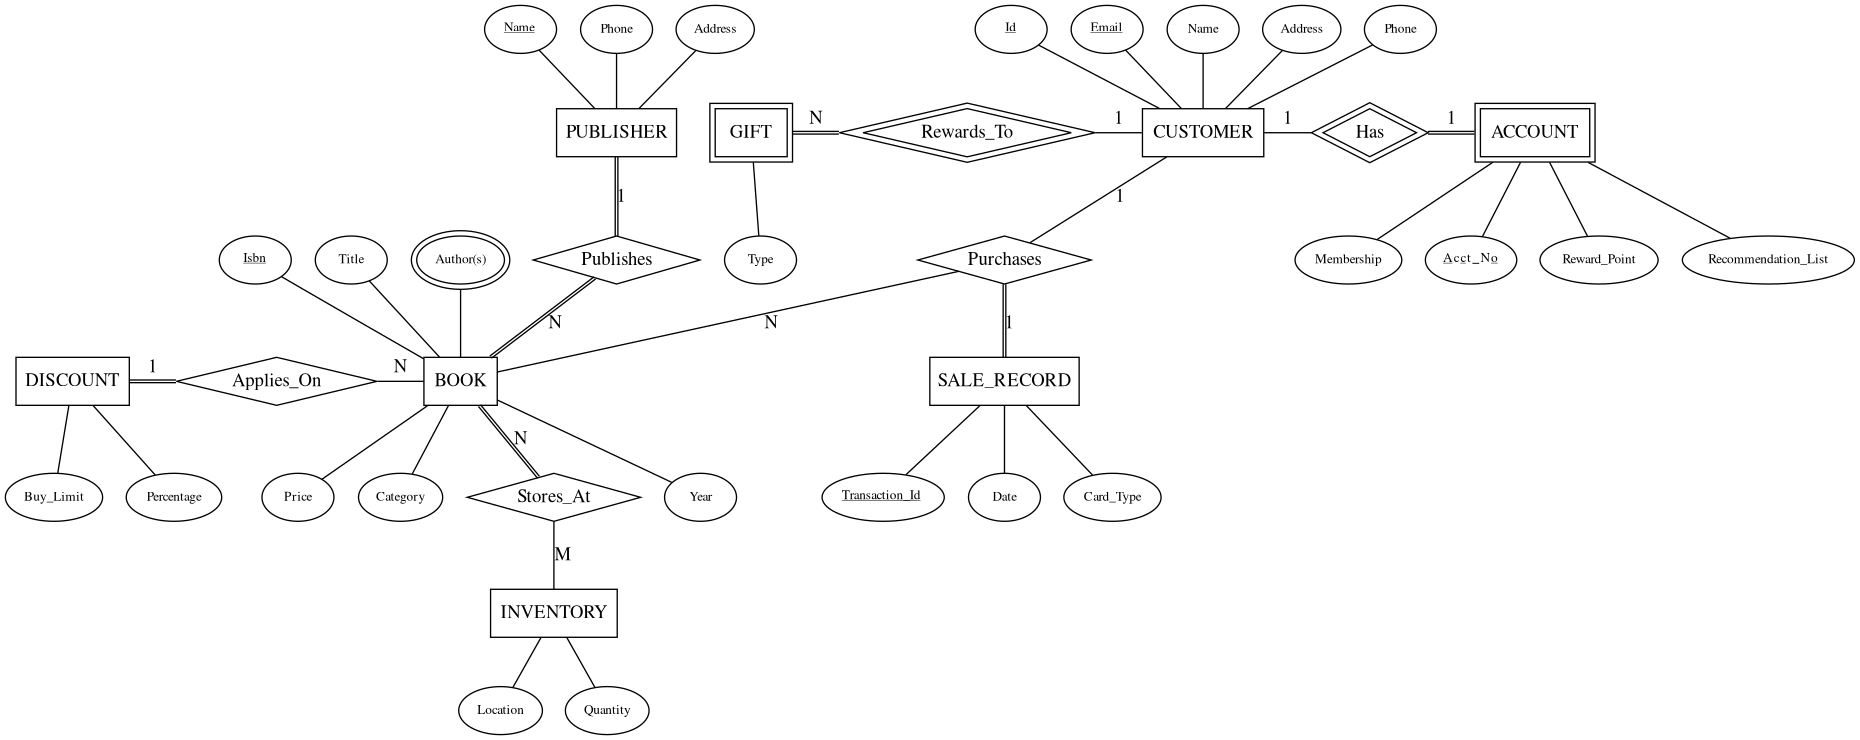
\includegraphics[width=\linewidth]{Section3/ER1.png}
\end{enumerate}

FIX:
\begin{enumerate}
\item Yes, we can.
\item See section 1, page 1 for updated ER model.
\item See section 1, page 1 for updated ER model.
\item See section 1, page 1 for updated ER model.
\item ID is removed, See section 1, page 1 for updated ER model.
\item Yes, it is.
\end{enumerate}

\subsection{Checkpoint 2}

\begin{enumerate}
\item Updated ER Model
  \begin{center}
    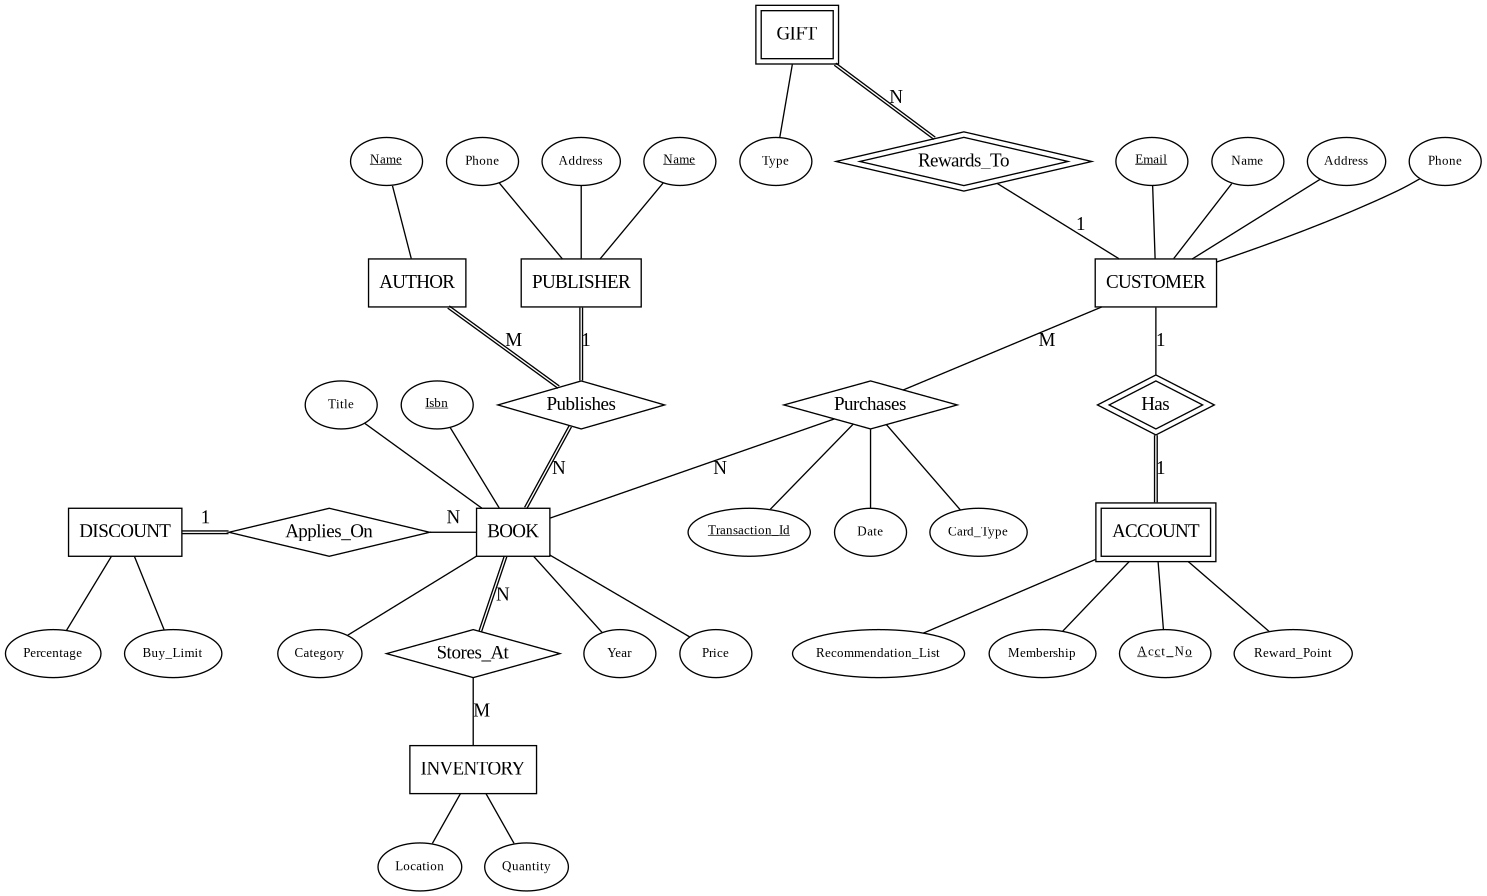
\includegraphics[width=\linewidth]{Section3/ER2.png}
  \end{center}

\item Relational Schema
  \begin{center}
    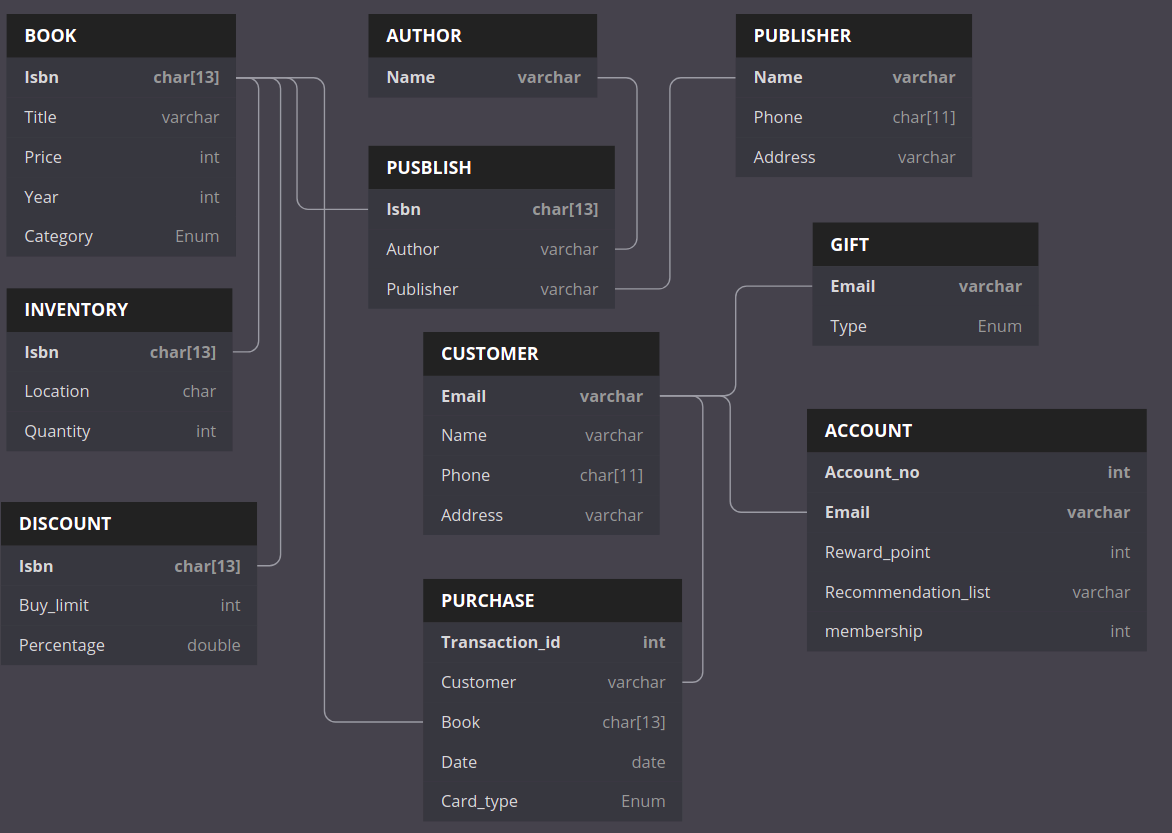
\includegraphics[width=\linewidth]{Section3/RS2.png}
  \end{center}

\item
  \begin{enumerate}

  \item Find the titles of all books by Pratchett that cost less than \$10
    \begin{equation*}
      \pi_{\textit{Title}}(\sigma_{\textit{Price} < 10}(BOOK))
    \end{equation*}

  \item Give all the titles and their dates of purchase made by a single
    customer (you choose how to designate the customer)\\
    designate CUSTOMER with Email
    \begin{align*}
      &\textit{BOOKS} \leftarrow \textit{BOOK} \bowtie_{\textit{Isbn} = \textit{Book}} (\sigma_{\textit{Customer}=\textit{Email}}(\textit{PURCHASE}))\\
      &\textit{RESULT} \leftarrow \pi_{Title, Date} (\textit{BOOK})
    \end{align*}

  \item Find the titles and ISBNs for all books with less than 5 copies in stock
    \begin{align*}
      &\textit{STOCK(Isbn, Quantity)} \leftarrow _{\textit{Isbn}}\mathcal{F}_{\textit{SUM Quantity}}(\textit{INVENTORY})\\
      &\textit{RESULT} \leftarrow \pi_{\textit{Title}, \textit{Isbn}}(\sigma_{\textit{Quantity} < 5}(STOCK))
    \end{align*}

  \item Give all the customers who purchased a book by Pratchett and the titles of Pratchett books they purchased
    \begin{align*}
      &\textit{PRATCHETTS} \leftarrow (\sigma_{\textit{Author} = \textit{Pratchett}}(\textit{PUBLISH}) * \textit{BOOK})\\
      &\textit{SALES} \leftarrow (\textit{PRATCHETTS} * \textit{PURCHASE})\\
      &\textit{RESULT} \leftarrow (\pi_{\textit{Email}, \textit{Name}, \textit{Title}}(\textit{SALES}))
    \end{align*}

  \item Find the total number of books purchased by a single customer (you choose how to designate the customer)
    \begin{align*}
      &\textit{COUNT(Customer, \# of Books)} \leftarrow _{\textit{Customer}}\mathcal{F}_{\textit{COUNT BOOK}}(\textit{PURCHASE})\\
      &\textit{RESULT} \leftarrow \sigma_{\textit{Customer} = \textit{Email}}(\textit{COUNT})
    \end{align*}

  \item Find the customer who has purchased the most books and the total number of books they have purchased
    \begin{align*}
      &\textit{COUNT(Customer, No)} \leftarrow _{\textit{Customer}}\mathcal{F}_{\textit{COUNT BOOK}}(\textit{PURCHASE})\\
      &\textit{RESULT} \leftarrow _{\textit{Customer}}\mathcal{F}_{\textit{MAX No}}(\textit{COUNT})
    \end{align*}

  \end{enumerate}

  \item
    \begin{enumerate}

    \item Find the CUSTOMER with the most Reward\_point on his/her account
    \begin{align*}
      &\textit{CACCT} \leftarrow \textit{CUSTOMER} * \textit{ACCOUNT}\\
      &\textit{RESULT} \leftarrow \pi_{\textit{Email, Name}}(_{\textit{Email, Name}}\mathcal{F}_{\textit{MAX Reward\_point}}(\textit{CACCT}))
    \end{align*}

  \item Find the most expensive BOOK with all the DISCOUNT applied
    \begin{align*}
      &\textit{DIS\_BOOKS} \leftarrow \textit{BOOK} \leftouterjoin \textit{DISCOUNT}\\
      &\textit{RESULT} \leftarrow _{\textit{Isbn, Title}}\mathcal{F}_{\textit{MAX} (\textit{Price} * \textit{percentage})}(\textit{DIS\_BOOKS})
    \end{align*}

  \item Find the total price of all the BOOK for each stock (quantity * price)
    \begin{align*}
      &\textit{STOCK} \leftarrow \textit{BOOK} * _{\textit{Isbn}}\mathcal{F}_{\textit{SUM Quantity}}(\textit{INVENTORY})\\
      &\textit{RESULT} \leftarrow \pi_{\textit{Isbn}, \textit{Quantity * Price}}(\textit{STOCK})
    \end{align*}

    \end{enumerate}

\end{enumerate}

FIX:
\begin{enumerate}
\item See section 1, page 1 for updated ER model.
\item See section 1, page 1 for updated ER model.
\item Primary Keys in ER diagram is marked with underline
\item See section 2, page 6 for updated relational algebra
\item There might be more than one INVENTORY, so it is
\item Checked
\end{enumerate}

\subsection{Checkpoint 3}

\subsubsection{Part 1}
\begin{itemize}
  \item Updated ER Model

    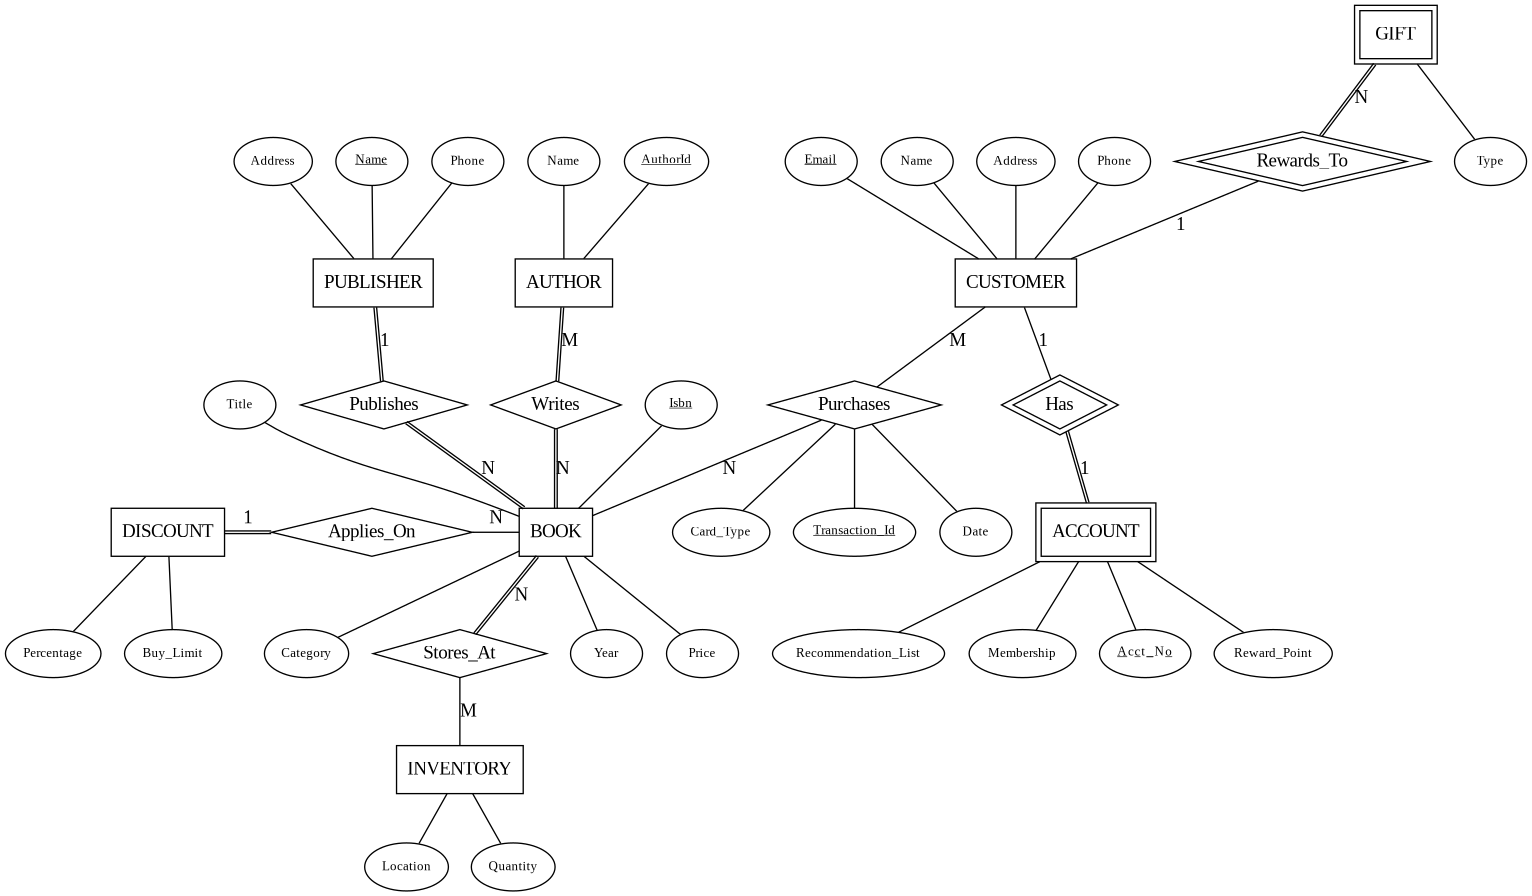
\includegraphics[width=\linewidth]{Section3/ER3.png}

  \item Updated Relational Schema

    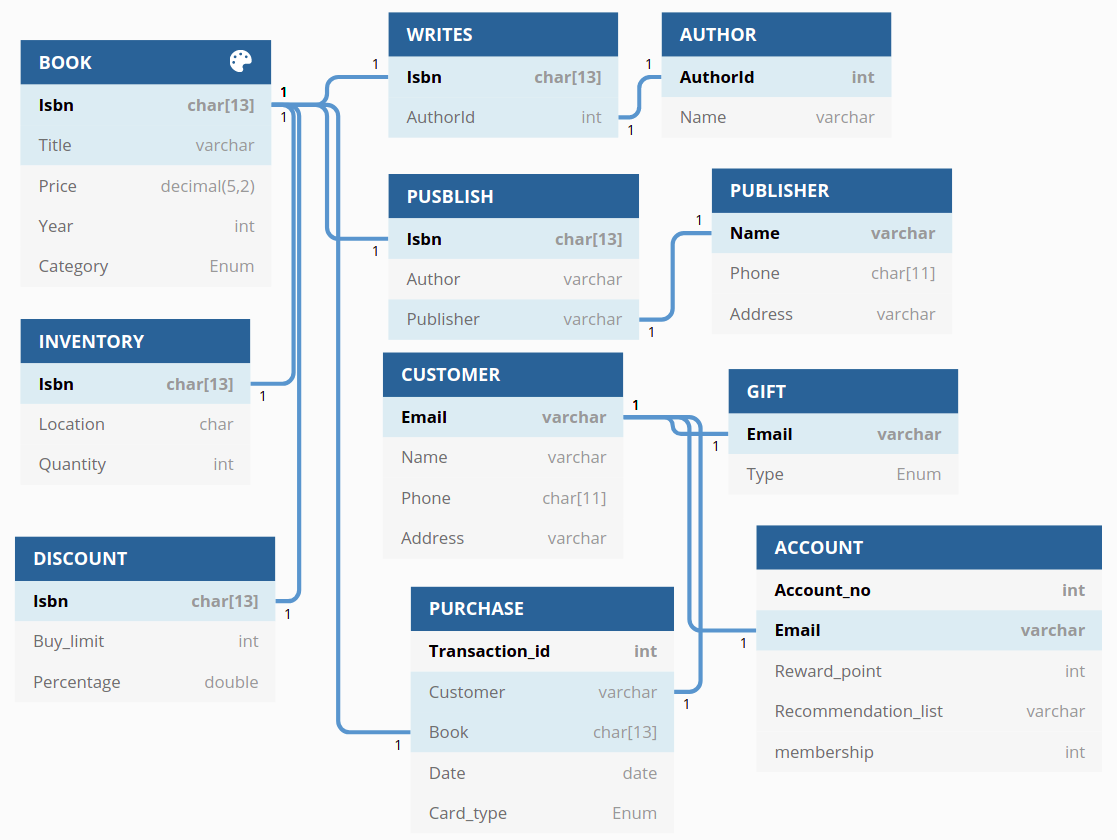
\includegraphics[scale=0.3]{Section3/RS3.png}
\end{itemize}

\subsubsection{Part 2}

\begin{enumerate}
  \item Question 1
  \inputminted[
  style=monokai,
  bgcolor=monokaibg,
  linenos]
  {sql}{Section3/Checkpoint3/Bookstore.sql}

  \item Question 2
    \inputminted[
    style=monokai,
    bgcolor=monokaibg,
    linenos]
    {sql}{Section3/Checkpoint3/WorkSheetTwoSimpleQueries.sql}

  \item Question 3
    \inputminted[
    style=monokai,
    bgcolor=monokaibg,
    linenos]
    {sql}{Section3/Checkpoint3/WorkSheetTwoExtraQueries.sql}

  \item Question 4
    \inputminted[
    style=monokai,
    bgcolor=monokaibg,
    linenos]
    {sql}{Section3/Checkpoint3/WorksheetTwoAdvancedQueries.sql}

\end{enumerate}

FIX:
\begin{enumerate}
  \item See section 2, page 6 for updated SQL
  \item See section 2, page 6 for updated SQL
  \item See section 2, page 6 for updated SQL
  \item See section 2, page 6 for updated SQL
  \item Checked
\end{enumerate}

\subsection{Checkpoint 4}
\begin{enumerate}
  \item Updated ER Model

    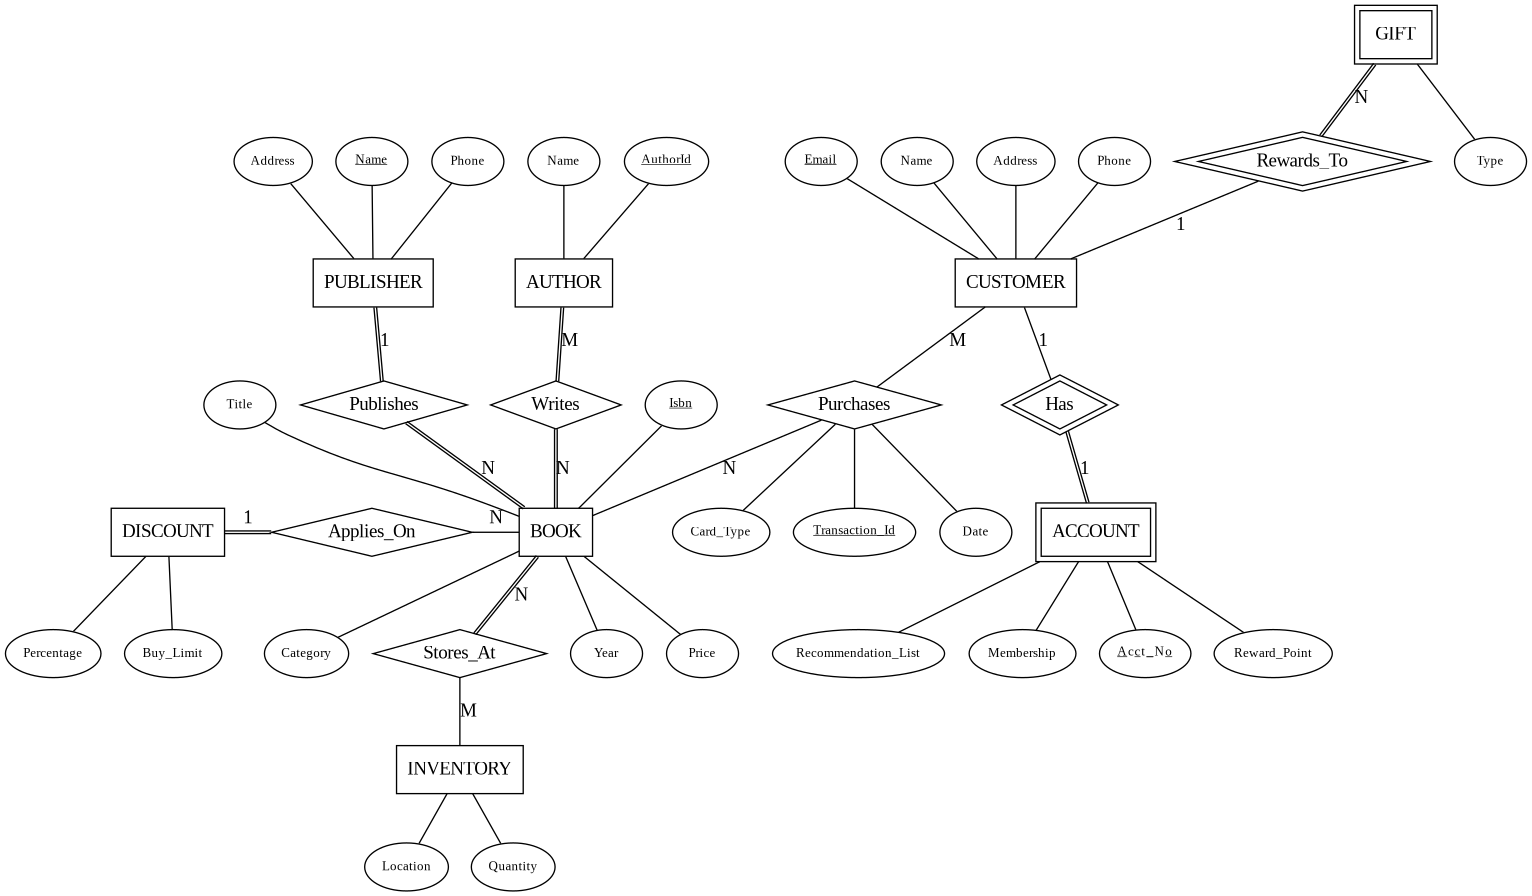
\includegraphics[width=\linewidth]{Section3/ER3.png}

  \item
    \begin{itemize}
    \item BOOK: \underline{Isbn} -> {Title, Year, Price, Category}
    \item PUBLISHER: \underline{Name} -> {Address, Phone}
    \item AUTHOR: \underline{AuthorId} -> Name
    \item CUSTOMER: \underline{Email} -> {Name, Address, Phone}
    \item ACCOUNT: \underline{Customer\_Email} -> {Membership, Reward\_Point, Recommandation\_List}
    \item PURCHASE: \underline{Transaction\_Id} -> {Customer, Book, Card\_type, Date}
    \item PUBLISHES: \underline{Isbn} -> {AuthorId, Publisher\_Name}
    \item WRITES: \underline{Isbn} -> \underline{AuthorId}
    \end{itemize}

  \item
    \begin{itemize}
      \item Book: BCNF
      \item Publisher: BCNF
      \item Author: BCNF
      \item Customer: BCNF
      \item Account: BCNF
      \item Purchases: BCNF
      \item Publishes: BCNF
      \item Writes: BCNF
    \end{itemize}

  \item N/A

  \item Two Views:
    \begin{enumerate}
    \item View A

      \inputminted[
      style=monokai,
      bgcolor=monokaibg,
      linenos]
      {sql}{Section3/Checkpoint4/view_a.sql}

    \item View B

      \inputminted[
      style=monokai,
      bgcolor=monokaibg,
      linenos]
      {sql}{Section3/Checkpoint4/view_b.sql}

    \end{enumerate}
\end{enumerate}

FIX:
N/A

\end{document}